\section{Gateway: Design \& Implementation}

\label{sec:gateway}
Having described our cryptographic building blocks, we can now discuss how they are used for encryption at the gateway.

\begin{figure}[t]
  \centering
  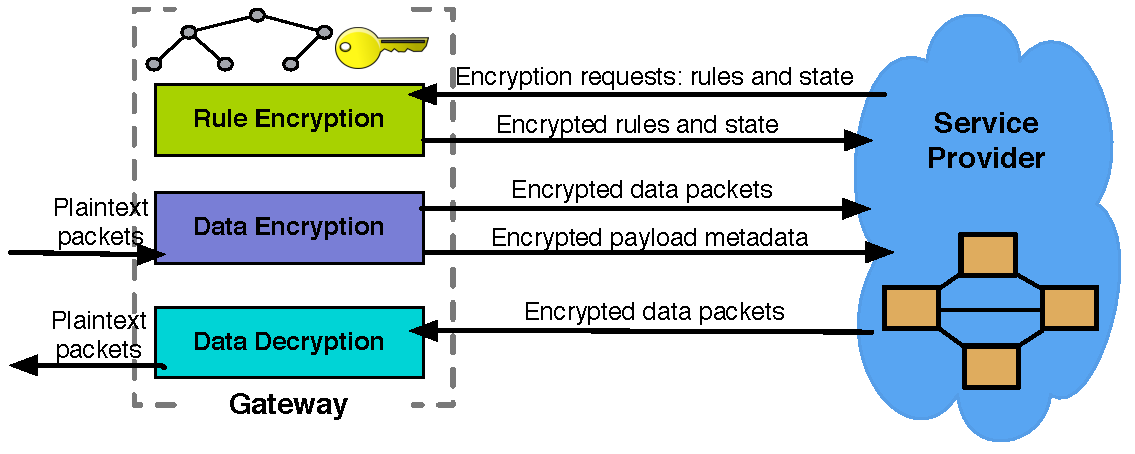
\includegraphics[width=3.25in]{fig/gateway2cloud}
  \caption[]{\label{fig:gatewaymeta} Communication between the cloud and gateway services: rule encryption, data encryption, and data decryption. \justine{Need to be consistent: is this a metadata channel or an extension channel}}
\end{figure}


\eat{
\begin{figure}[t]
  \centering
  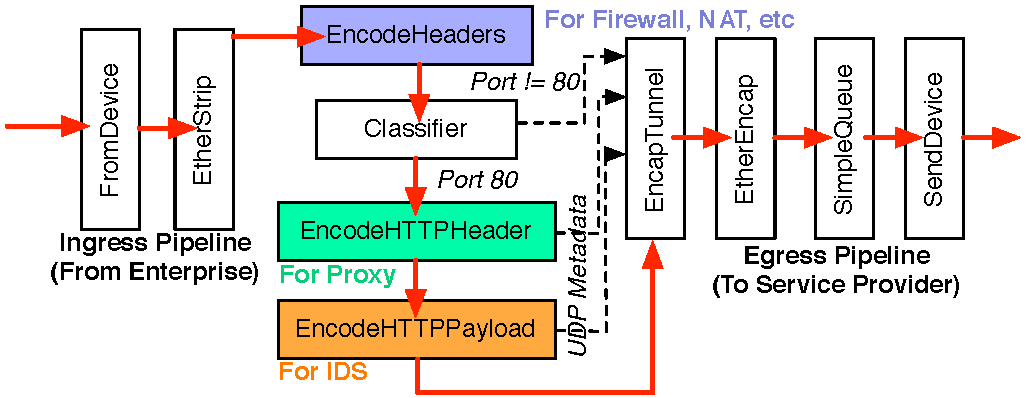
\includegraphics[width=3.25in]{fig/gatewaydiag}
  \caption[]{\label{fig:gateway} Data encryption (enterprise to cloud) click module.}
\end{figure}
}

The gateway serves two purposes. First, it redirects traffic to/from the cloud for middlebox processing. Second, it provides the cloud with encryptions of IDS/FW rulesets and updates to the RangeMatch tree.
Every gateway is configured statically to tunnel traffic to a fixed IP address at a single service provider point of presence.
A gateway can be logically thought of as three services: the rule encryption service, the pipeline from the enterprise to the cloud (Data encryption), and the pipeline from the cloud to the enterprise (Data decryption). 
All three services share access to the RangeMatch tree and the private key $k$.
Figure~\ref{fig:gatewaymeta} illustrates  these three services and the data they send to and from the cloud provider.

We design the gateway with two design principles in mind: 

\noindent{\bf Format-compatibility}: in converting plaintext traffic to encrypted traffic, the encrypted data should be structured in such a way that the traffic {\it appears as normal IPv6 traffic} to middleboxes performing the processing. This allows us to leave many middleboxes completely unmodified in how they perform per-packet operations, ensuring compatibility with optimizations including those in hardware (and hence good performance at the cloud). 

\noindent{\bf Low Complexity and Scalability}: the gateway should perform only inexpensive per-packet operations and should be parallelizable. The gateway should not require configuration other than to generate a key and establish a session with the cloud provider. If the gateway were as expensive and complex as the middleboxes themselves, the client would have no cost or management benefits from outsourcing. 

We now discuss how the gateway performs encryption and decryption (\S\ref{sec:dataenc}) and how rules are encrypted (\S\ref{sec:rulenc}) with these design goals in mind.

\subsection{Data Encryption and Decryption}
\label{sec:dataenc}

As shown in Table~\ref{tbl:mbreqs}, we categorize middleboxes as Header middleboxes, which operate only on IP and transport headers; HTTP middleboxes, which operate on HTTP headers and may operate on IP and transport headers; and DPI middleboxes, which operate on arbitrary fields in a connection bytestream. 
We discuss how each category of data is encrypted/decrypted in order to meet middlebox requirements as follows.

\subsubsection{IP and Transport Headers}
IP and Transport Headers are encrypted field by field (\eg{}, a source address in an input packet results in an encrypted source address field in the output packet) with RangeMatch.
We use RangeMatch for these fields because many middleboxes perform analysis over prefixes and ranges of values -- e.g., a firewall may block all connections from a restricted IP prefix.

\noindent{\bf Decryption.} RangeMatch is not reversible. To enable packet decryption, We store the AES encrypted values for the header fields in the IP options header. When the gateway receives a packet to decrypt, it decrypts the values from the options header restores them to the IP or transport header.

\noindent{\bf Format-compatibility.} 
Our modifications to the IP and transport headers place the encrypted range match data back in to the same fields as the unencrypted data was originally stored; because comparisons between rules and encrypted data rely on $\leq$ $\geq$, just as unencrypted data, this means that operations performing comparisons on IP and transport headers {\it remain entirely unchanged at the middlebox.}
Not only does this ensure backwards-compatibility with existing software {\it and hardware} dataplane operations -- because per-packet operations are tightly optimized in production middleboxes, this compatibility ensures good performance at the cloud despite our changes.

An additional challenge for format compatibility is where to place the decryptable AES data; one option would be to define our own packet format, but this could potentially lead to incompatibilities with existing middlebox software. By placing it in the IPv6 options header, middleboxes can be configured to ignore this data using standard configuration.\footnote{It is a common misconception that middleboxes are incompatible with IP options. Many middleboxes deployed on the Internet are aware of IP options but {\it configured} to filter or drop them. Our cloud provider would have to {\it configure} the middleboxes to ignore the options, but industrial middleboxes would not require new code to handle an unexpected, new packet format.}


\subsubsection{Payload Data} 
Payload Data is encrypted with KeywordMatch using a searchable encryption approach (we discuss this in detail in \S\ref{sec:gateway}). This allows \sys to support DPI middleboxes, such as intrusion detection or exfiltration prevention.
These devices must detect whether or not there exists an exact match for an encrypted rule string {\it anywhere} in the connection bytestream.
The gateway transmits the encrypted bytestream over an `extension', secondary channel that only those middleboxes which perform DPI operations inspect. 
Other middleboxes ignore this extra data.

Importantly, because this encrypted payload data is over the {\it bytestream}, we need to generate encrypted values which span `between' packets. Searchable Encryption schemes, which we use for encrypted DPI, require that traffic be {\it tokenized} and that a set of fixed length substrings of traffic be encrypted along a sliding window -- e.g., the word malicious might be tokenized into {'malici', 'alicio', 'liciou', 'icious'}.
If the term 'malicious' is divided across two packets, we may not be able to tokenize it properly unless we reconstruct the TCP bytestream at the gateway. Hence, if DPI is enabled at the cloud, we do exactly this.

\noindent{\bf Decryption.} The payload data is encrypted with AES and placed back into the packet payload -- like RangeMatch, KeywordMatch is not reversible and we require this data for decryption at the gateway.
Because the extension channel is not necessary for decryption, it is not transmitted back to the gateway.

\noindent{\bf Format-compatibility.} To middleboxes which only inspect/modify packet headers, encrypting payloads has no impact. Once again we are still faced with the challenge of where to place the extra data, however, with the KeywordMatch values. By placing this data in the extension channel, the extra traffic can be routed past and ignored by middleboxes which do not need to operate over this data, hence it will not interfere with normal processing. 

DPI middleboxes which do inspect payloads must be modified to inspect the extension channel alongside the primary channel, as described in~\cite{blindbox}; as we show in \S\ref{sec:eval}, DPI devices are typically implemented in software rather than hardware and our modifications to them to inspect the extension channel rather than the primary impose modest throughput overhead. 

\subsubsection{HTTP Headers} 

HTTP Headers are a special case of payload data.
Middleboxes such as proxies, L7 load balancers, and parental filters do not read arbitrary values from packet payloads: the only values they read are the HTTP headers.
We treat these values specially compared to other payload data; we encrypt the HTTP URI using unsalted AES (which is deterministic) and store them in IP options header of the packet containing the request.

This optimization is useful for two reasons. First, so many middleboxes inspect HTTP headers that it does not make sense for them to parse entire packet bytestreams -- as generated in the extension channel -- because we are scanning through the traffic at the gateway already is makes sense to mark these fields specially.
Second, when DPI is not enabled, we can extract and store the HTTP headers statelessly; so long as HTTP pipelining is disabled and packet MTUs are standard-sized (>1KB), the required fields will always appear contiguously within a single packet.
Hence, if DPI is disabled we can avoid reconstructing the TCP bytestream at the middlebox.

\noindent{\bf Decryption.} The packet is decrypted as normal using the data stored in the payload; options are removed.

\noindent{\bf Format-compatibility.}
Once again, by placing the encrypted value in an IP options header, we can avoid conflicts that arise from defining our own protocol.
We do need to rewrite HTTP parsing devices but, like DPI devices, they are implemented in software and our modifications introduce no overhead (as discussed in \S\ref{sec:eval}).


\subsection{Rule Encryption}
\label{sec:rulenc}
\justine{lock here -- currently editing!}

The rule encryption component provides the cloud provider with encrypted rules/policies to use at the middlebox. 
There are two possible ways rules can be generated. First, an enterprise may choose to generate their own rules, in which case, they send encrypted versions of the rules directly to the cloud.
Alternately, the enterprise may opt in to a `default' set of rules from the cloud provider, in which case the cloud provider sends the rules to the gateway which encrypts them and sends them back.
Rules can contain IP and transport header values -- which must be encrypted with RangeMatch -- or HTTP header fields, or DPI signatures, which must be encrypted with KeywordMatch.

The rule encryption component also handles rule updates. 
Whenever an adjustment is made to the RangeMatch table, it sends an update to the cloud provider with the adjusted mappings/rules.
If the gateway ever changes its key, the encryption component must also signal to the cloud provider and re-encrypt all rules.


\subsection{Discussion}
\label{sec:gwdiscuss}
\textbf{Scalability}
\textbf{Complexity}
\textbf{Fault Tolerance}
